\documentclass[a4paper,oneside]{alpenthesis/alpenthesis}
% <<< Preamble
\hexfalse
\paperfalse
%https://tex.stackexchange.com/a/210456/131649
\renewcommand\partnumberlinebox[2]{#2\hspace{2em}}
\usetikzlibrary{positioning}
% >>>
\begin{document}
\begin{titlingpage} % <<<
    \fullhexpage{q1}{q0}
    \flushright\sffamily

    \vspace*{5em}
    \Huge\bfseries{Red Pitaya}\\[1ex]
    \Large\mdseries{Thesis}\\[3ex]

    \normalsize\mdseries
    
    \vfill
    Raphael Frey\\
    Noah H\"usser\\[3ex]

    \vspace{5em}

    \today\\
    Version 0.0.1
\end{titlingpage} % >>>

\frontmatter % <<<
\tableofcontents*
% >>>

\mainmatter

\chapter{Introduction} % <<< ------------------------------------------------- %
\label{ch:intro}
% ---------------------------------------------------------------------------- %

\begin{itemize}\firmlist
    \item Rationale (Why?)
    \item What is the general approach to solve this problem?
    \item What has been done so far?
    \item Results of previous work
    \item What are we going to do?
    \item What are the contents of this report?
\end{itemize}

% >>>

\part{System Overview} % <<< ------------------------------------------------- %
\label{part:System_Overview}
% ---------------------------------------------------------------------------- %

Fundamental question  to answer in  this part:  \emph{What is our  system, and
what is it good for?}

This information could also go into \emph{Introduction}?

Provide supplementary theoretical background as needed.

\chapter{Analog-to-Digital Data Acquisition} % <<< --------------------------- %
\label{ch:analog-to-digital_data_aquisition}
% ---------------------------------------------------------------------------- %

\begin{itemize}
    \item
    Generic Chapter on some of the basic principles of AD data processing
    \item 
    Very brief mention of aliasing, low-pass filtering and all that
    \item
    Oversampling and Downsampling
    \item
    Oversampling: Explain advantage w/r to SNR
    \item
    Fancy graphics from Mr. Gut
    \item
    How does the Red Pitaya fit into this?
    \item
    CIC and FIR filters:
        \begin{itemize}
            \item
            Overview (emphasis on CIC)
            \item
            Where to use which, and why?
            \item
            Table/Matrix with advantages and drawbacks for each
            \item
            How does this translate to our system/Why is this important for us?
        \end{itemize}
\end{itemize}

Explain processing chain (do we even have an analog LP filter here?)

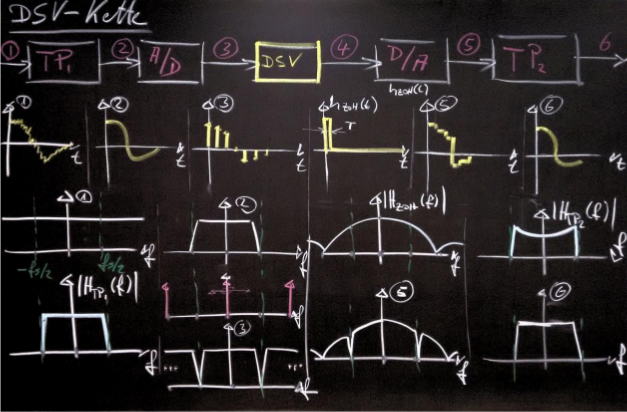
\includegraphics[width=0.75\textwidth]{images/dsvChain}

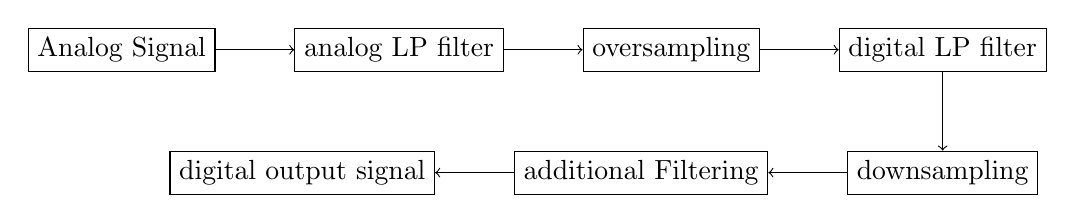
\begin{tikzpicture}[
        every node/.style={draw}
    ]
    \node (analog) at (0,0) {Analog Signal};
    \node[right=of analog] (lpf) {analog LP filter};
    \node[right=of lpf] (sampling1) {oversampling};
    \node[right=of sampling1] (lpf2) {digital LP filter};
    \node[below=of lpf2] (downsampling) {downsampling};
    \node[left=of downsampling] (addf) {additional Filtering};
    \node[left=of addf] (digital) {digital output signal};

    \draw[->] (analog) -- (lpf);
    \draw[->] (lpf) -- (sampling1);
    \draw[->] (sampling1) -- (lpf2);
    \draw[->] (lpf2) -- (downsampling);
    \draw[->] (downsampling) -- (addf);
    \draw[->] (addf) -- (digital);
\end{tikzpicture}

% >>>

\chapter{The Red Pitaya Platform} % <<< -------------------------------------- %
\label{ch:the_red_pitaya_platform}
% ---------------------------------------------------------------------------- %
\section{General Information}
General Info about Red Pitaya Project:
\begin{itemize}\firmlist
    \item How is the PITA project structured? (logically, license-wise, philosophically)
    \item Why do we care about this?
    \item Replacement for scopes (motivation: Why would one use the PITA?)
\end{itemize}
\subsection{FPGA}
\subsection{Linux}

\section{Performance and Possible Improvements}
\begin{itemize}
    \item
    What is the stock solution for downsampling and such? Performance?
    \item
    Results of Previous Work
    \item
    Consequences for us: Possible paths forward
    \item
    System Analysis
    \item Decision Matrix \& Decision
\end{itemize}

% >>>

% >>>

\part{Implementation} % <<< -------------------------------------------------- %
\label{part:Implementation}
% ---------------------------------------------------------------------------- %
Implementation can be read independently of previous part, but there should be
a  red thread  from decision  to implementation. Deals  primarily with  design
decisions.

Present a diagram with all  system components. Then document the components in
their respective chapters and sections.

\chapter{Data Acquisition System}
\label{ch:data_acquisition_system}
\section{FPGA}
\section{Kernel Module}

\chapter{Filters} % <<< ------------------------------------------------------ %
\label{ch:filters}
% ---------------------------------------------------------------------------- %

% >>>

\chapter{Server} % <<< ------------------------------------------------------- %
\label{ch:server}
% ---------------------------------------------------------------------------- %

% >>>

\chapter{Graphical Front End} % <<< ------------------------------------------ %
\label{ch:graphical_front_end}

% >>>

% >>>

\part{Developer Guide} % <<< -------------------------------------------------- %
\label{part:Developer_Guide}
% ---------------------------------------------------------------------------- %
Documentation for a person who wishes to utilize our system in their work and/or
improve upon it?

Make sure  to distinguish  between \emph{Implementation} and  this part. Lines
seem a bit blurry to me (R.F.) at the moment (\today).

\chapter{IP Core} % <<< ------------------------------------------------------ %
\label{ch:IP_Core}
% ---------------------------------------------------------------------------- %
Documentation of our FPGA Project (structure, interfaces, registers \ldots)

% >>>

\chapter{Linux} % <<< -------------------------------------------------------- %
\label{ch:Linux}
% ---------------------------------------------------------------------------- %

Kernel module, server

% >>>

\chapter{Tool Chain} % <<< --------------------------------------------------- %
\label{ch:Tool_Chain}
% ---------------------------------------------------------------------------- %
Vivado, Build Box, ARM Linux, TCL, Makefiles, Libs for building server application

% >>>

% >>>

\part{User Guide} % <<< ------------------------------------------------------ %
\label{part:User_Guide}
% ---------------------------------------------------------------------------- %
Documentation for the end user. Primarily concerned with the scope front-end.

% >>>

\end{document}
%^^A vim: foldenable foldcolumn=4 foldmethod=marker foldmarker=<<<,>>>
